\section{Hastighedsregulerende kreds}
\begin{figure}[H]	\label{kreds:hastighed}
	\centering
    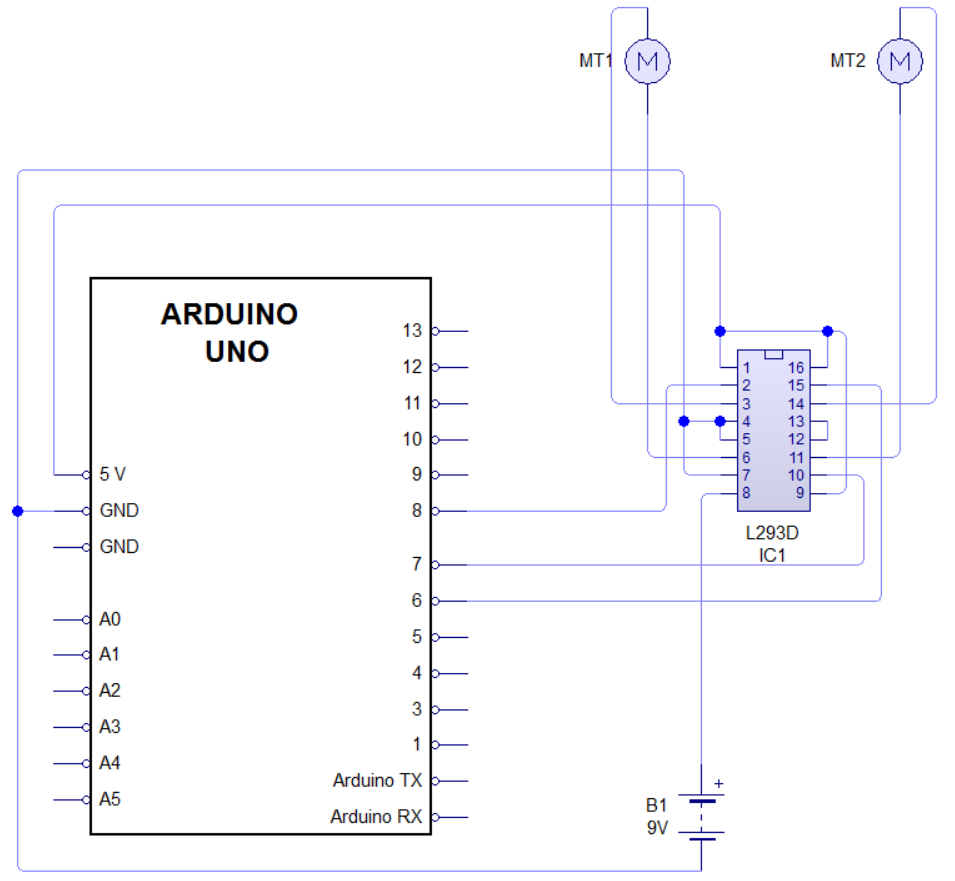
\includegraphics[width=10cm]{figures/2_4kredse/hastighed.png}
	\caption{Et billede af kredsløbet for den hastighedsregulerende kreds.}
\end{figure}
Som der kan ses på Figur \ref{kreds:hastighed}, er der motorene MT1 og MT2. Heraf gælder det at MT2 fungerer som et gear og MT1 fungerer som selve elastik-optrækkeren. Når motoren trækkes op løber der først strøm fra Arduinoens pin 6 
 %*** eller pin 6?
 hvorfra gennem L293D pin 14 kan strøm løbe gennem MT2 og låse gearet fast. Derefter sendes der strøm gennem Arduinoens pin 8 som trækker MT1 op. 
Til sidst slukkes for signalet til MT1 og derefter ændres polariteten i MT2, så affyringsmekanismen er i ``frigear''. Det skal således bemærkes at MT2 modtager 2 signaler fra arduinoen for at kunne vende polariteten.

\subsection{Komponenter}
\subsection{Lego $\SI{9}{V}$ DC motor}
Vi kunne ikke finde et specifik datablad, men vi ved at normal lego-mindstorm DC motor der kører på $\SI{9}{V}$, hvilket er fint til vores formål. 
\subsection{Dual H-bridge motor driver - L293D}
\begin{figure}[H] \label{fig:pindiagramL293D}
	\centering 
    \frame{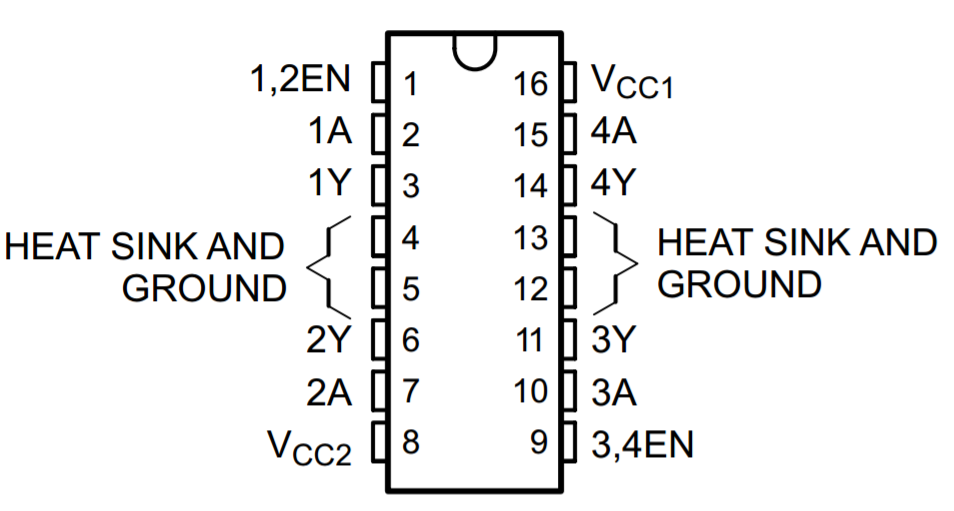
\includegraphics[width=10cm]{figures/komponenter/L293D.png}}
	\caption{Pindiagram af L293D}
\end{figure}
Pindiagram kan ses på Figur \ref{fig:pindiagramL293D}. Pin 1 og 9 er aktiverings pins for H broerne. Pin 1 aktiverer H broen på venstre side og pin 9 aktiverer H broen på højre side. Pin 2 og 7 bruges til at styre motoren koblet til 3 og 6. Pin 10 og 15 styre motoren på 11 og 14. Pin 4,5,13 og 12 er forbundet, og skal forbindes til jord. Kilde for komponentet: \cite{komphbridge}.
\subsection{Teori}
% \subsubsection{DC motor} *** Måske skriv
\subsubsection{H bridge}
En H-bridge er et komponent der benyttes til at vende polariteten i vores DC-motor som fungerer som gear. Dette gøres overordnet ved at H-formede kredse med switches der kan enten være on eller off. 
\begin{figure}[H]
	\centering
    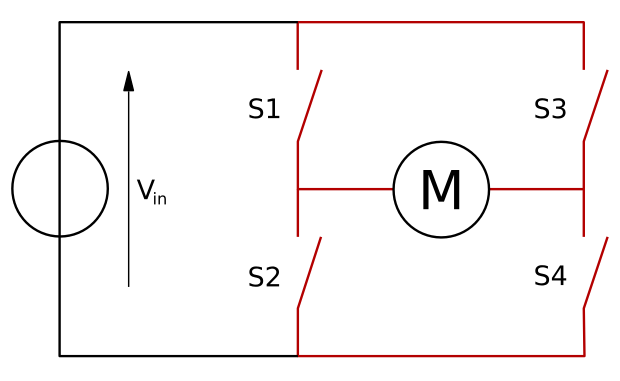
\includegraphics[width=13cm]{figures/2_4_3hastighed/hbridge.png}
	\caption{Et billede af en H-bridge, selve H-bridge struturet er markeret med rød. Kilde: \cite{teorihbridge}}
	\label{fig:hbridge}
\end{figure}
Det fremgår på Figur \ref{fig:hbridge} at switchene 1 til 4 er åbne. Disse switches kan så hvis de modtager et signal kan man forbindes således at strømmens retning løber i en bestemt retning. F.eks. Hvis S1 og S4 er lukkede switches, vil motoren løbe i en retning, end hvis S3 og S2 er lukkede switches. Kilde: \cite{teorihbridge}. 

%\subsection{Beregninger}

\subsection{Test}
\todo{Vi skal not beskrive hvordan vi testede denne kreds og have noget kode på det. ***}